% \begin{savequote}[75mm]
% Nulla facilisi. In vel sem. Morbi id urna in diam dignissim feugiat. Proin molestie tortor eu velit. Aliquam erat volutpat. Nullam ultrices, diam tempus vulputate egestas, eros pede varius leo.
% \qauthor{Quoteauthor Lastname}
% \end{savequote}

\chapter{Nonlinear Interaction Networks}



Hawkes process inference relied on an augmentation strategy 
made possible by the linear form and excitatory nature 
 of the interactions. In neural settings, these assumptions 
of the Hawkes process are not as realistic. Instead, we turn to 
the nonlinear Hawkes process, which allows for both excitatory 
and inhibitory interactions by introducing a nonlinearity 
into the model. This corresponds to the popular generalized 
linear model that is widely used in computational neuroscience. 
We develop a novel approach that leverages the 
\polyagamma augmentation to enable efficient, fully-conjugate 
inference. Again, we combine the nonlinear Hawkes process with 
prior distributions on the network of interactions, and we focus 
on a discrete time approximation. This is part of ongoing work 
with Ryan and Jonathan Pillow at Princeton, and it has grown out 
of a Cosyne abstract \cite{linderman2015cosyne}. I also have an 
unpublished draft in which I extend the abstract and apply it 
to a variety of neural datasets, and show how the network models 
recover interesting latent features like neural types and locations.
I will submit a journal version of this paper as soon as possible.

\section{Abstract} 
We develop a novel method for the unsupervised discovery of interpretable latent structure underlying neural recordings. 
Rather than directly clustering or factorizing measured activity, we propose a generative model that links latent clusters and features of neurons to measured activity via an intermediate functional network. 
Thus, latent structure is defined in terms of how neurons interact with one another rather than how they behave. 
To discover the most appropriate structural form, we propose a fully-Bayesian inference algorithm that enables efficient inference and principled model comparison. 
We demonstrate the efficacy of this approach on synthetic data and simultaneously recorded multi-neuronal spike trains.


\section{Introduction}
As our neural recording capabilities are rapidly expanded, the need for automated methods of exploring large-scale multineuronal recordings becomes ever more pressing. 
Though our recordings may be incomprehensibly large, capturing the activity of hundreds of thousands of neurons for hours or days at a time, the underlying neural population often exhibits some simplifying structure. 
For example, we commonly find low-dimensional continuous embeddings of neural populations using tools like principal components analysis (PCA), or distinct classes of neurons with clustering algorithms like k-means. 
These simplified representations serve a number of roles: 
they reduce data to a interpretable set of features and types; 
they denoise data by capturing shared structure and throwing away noise; 
they may confirm that hypothesized structure exist, for example, that spatially localized cells are functionally similar as well; 
and, most importantly, they suggest novel hypotheses about how neural populations should be understood.

\TODO{Discuss some recent successes of unsupervised structure discovery methods and emphasize some examples of continuous and discrete representations}

Unfortunately, most common approaches do not take advantage of the important temporal dependencies in neural recordings. 
The generative assumptions underlying PCA assert that each neuron's activity can be represented as a linear combination of a small number of bases. 
It says nothing about the relationship between activity in one time bin and the next.
Similarly, na\"ive clustering methods implicitly assume that time bins are conditionally independent given the latent cluster assignment. 
We propose a generative model where latent structure is reflected in an patterns of functional connectivity among neurons.  This functional network parameterizes an autoregressive model that gives rise to temporally structured activity.
  
Figure~\ref{fig:fig1} illustrates the steps of the proposed generative model. 
We assume that neuron~$n$ has some latent feature~$z_n$ that may be continuous or discrete. 
In Figure~\ref{fig:fig1}, each neuron belongs to one of four classes, so~$z_n$ is discrete and is one of~$\{\textit{red}, \textit{blue}, \textit{green}, \textit{yellow}\}$. 
These latent class assignments affect the probability of a functional connection from one neuron to another. 
In this case, \textit{red} neurons sparsely connect to \textit{blue} neurons, \textit{blue} to \textit{green}, and \textit{green} to \textit{yellow}.
These connections are aggregated into the functional network,~$\bW$, shown in Figure~\ref{fig:fig1}.
Finally, this network parameterizes an autoregressive model for neural activity.
In this case, the \textit{activation} of the~$n$-th neuron,~$\psi_n(t)$, depends on the number of spikes that connected neurons fired in the preceeding time bins. 
%This might give rise to the roughly periodic activity shown in Figure~\ref{fig:fig1}.

This generative approach formalizes many of the intuitive hypotheses that systems neuroscientists already employ. 
Neural circuits are commonly described with simplified block diagrams that show how one subpopulation of neurons drives another. 
In other cases, neurons are described by continuous features, such as ``place fields'' that describe the spatial location in which hippocampal place cells fire.
Since our movement is continuous, neurons with similar place fields are functionally correlated.
Our approach begins with high-level hypotheses like, ``neurons have latent types that determine functional connectivity.''
These hypotheses are instantiated as generative models which are then fit to the data using probabilistic inference techniques and compared on the basis of how well they explain the measured activity.

We show how a host of high-level hypotheses can be formalized as generative models using random network models. 
We then develop a flexible Bayesian inference algorithm for discovering the latent parameters of this model from the measured activity. 
Finally, we derive a principled method for comparing these models on the basis of their \textit{marginal likelihood}, that is, the probability they assign to the data. 
We demonstrate the efficacy of this approach on both synthetic and real-world datasets. 

% \begin{figure}[t]
%   \centering
%   \begin{subfigure}[b]{.3\textwidth}
%     \centering
%     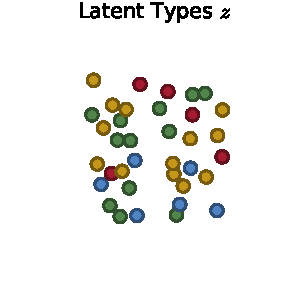
\includegraphics[width=\textwidth]{clustered_neurons}
%     \caption{}
%     \label{fig:fig1_z}
%   \end{subfigure}
%   \begin{subfigure}[b]{.3\textwidth}
%     \centering
%     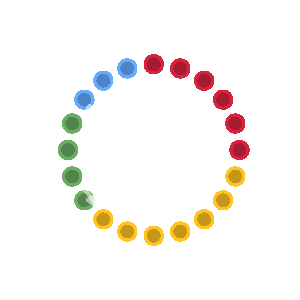
\includegraphics[width=\textwidth]{clustered_network}
%     \caption{}
%     \label{fig:fig1_W}
%   \end{subfigure}
%   \begin{subfigure}[b]{.3\textwidth}
%     \centering
%     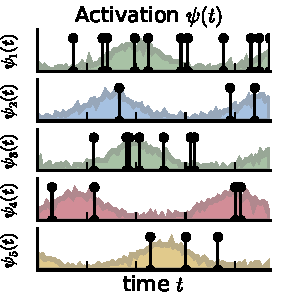
\includegraphics[width=\textwidth]{clustered_rates}
%     \caption{}
%     \label{fig:fig1_psi}
%   \end{subfigure}
%   \caption{Illustrative example of a generative model relating latent
%     structure to multineuronal spike trains via a functional
%     network. (a) Here, neurons have a latent class (\textit{red},
%     \textit{blue}, \textit{yellow}, or \textit{green}). 
%     (b) These classes govern the probability of functional
%     interactions for each pair of neurons. (c) The network
%     parameterizes an autoregressive model for the activation of the
%     neurons, which, in this example, give rise to the stochastic spike
%     trains we observe.}
% \label{fig:fig1}
% \end{figure}


\begin{figure}[t]
  \centering
  \begin{subfigure}[b]{\textwidth}
    \centering
    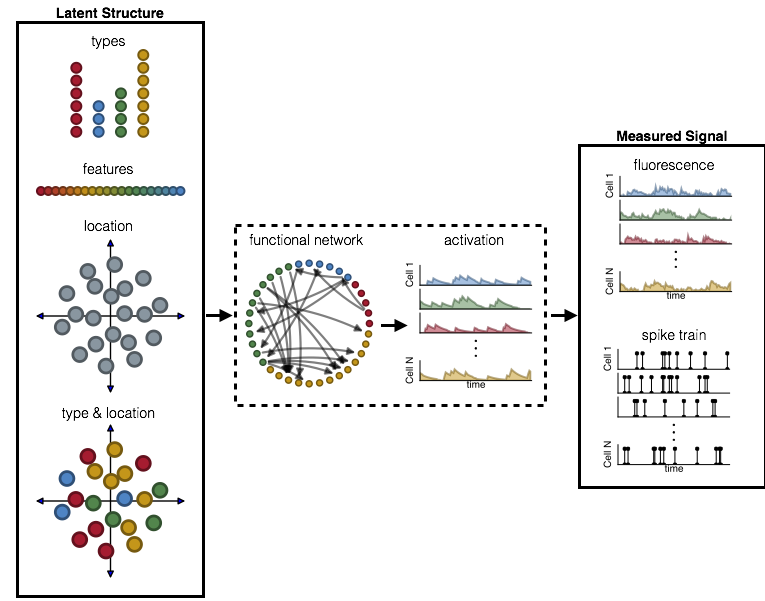
\includegraphics[width=\textwidth]{figures/ch3/figure1.png}
  \end{subfigure}
  \caption{Overview of model.}
  \label{fig:fig1}
\end{figure}

\section{Results}

\subsection{Retinal Ganglion Cells}

\subsection{Hippocampal Place Cells}

\subsection{Calcium Fluorescence}

\section{Methods}
Our primary contribution is a novel framework for discovering latent
network structure underlying neural activity.  This framework consists
of a probabilistic model relating structure to observed signals, an
efficient Bayesian inference algorithm capable of fitting this model,
and a model selection algorithm that enables principled comparison of
structural forms.

\subsection{Probabilistic Model}
A probabilistic model specifies a joint probability distribution over
measured signals, the underlying network, and latent structural
variables we wish to infer.  In our model, the measured signal from
neuron~$n$ in the~$t$-th time bin is denoted~$s_{t,n}$, which may 
denote either a discrete spike count or a real-valued signal, like 
the calcium fluorescence. In either case, this signal is assumed 
to be stochastically drawn from a distribution parameterized by 
an underlying, real-valued \emph{activation},~$\psi_{t,n}$,
and a static parameter,~$\nu_n$. The
activation is typically related to the expected spike count via
a logistic transformation,~$\sigma(\psi) = e^\psi \, (1+e^\psi)^{-1}$,
which has the property~$\sigma(-\psi) = 1-\sigma(\psi)$.

\begin{table}
\begin{center}
\begin{tabular}{c|c|c|c|c}
  \textbf{Distribution} & $p(s \given \psi, \nu)$ & Standard Form & $\bbE[s]$ & $\Var(s)$ \\
  \hline
  Gaussian & $\frac{1}{\sqrt{2 \pi \nu}}\exp \left \{ -\frac{1}{2 \nu} (s - \psi)^2 \right \}$
  & --- 
  & $\psi$ & $\nu$ \\
  Bernoulli & $\sigma(\psi)^s \, \sigma(-\psi)^{1-s}$
  & $\frac{(e^\psi)^s}{1+e^\psi}$
  & $\sigma(\psi)$ & $\sigma(\psi) \, \sigma(-\psi)$ \\
  Binomial & ${\nu \choose s} \, \sigma(\psi)^s \, \sigma(-\psi)^{\nu-s}$
  & ${\nu \choose s} \,\frac{(e^\psi)^s}{(1+e^\psi)^\nu}$
  & $\nu \sigma(\psi)$ & $\nu \sigma(\psi) \, \sigma(-\psi)$ \\
  Neg. Binomial & ${\nu + s -1 \choose s} \, \sigma(\psi)^s \, \sigma(-\psi)^{\nu}$
  & ${\nu +s - 1 \choose s} \,\frac{(e^\psi)^s}{(1+e^\psi)^{\nu+s}}$
  & $\nu e^\psi$ & $\nu e^\psi / \sigma(-\psi)$ \\
\end{tabular}
\end{center}
\caption{List of observation distributions.}
\label{tab:obs_models}
\end{table}

We consider the four observation models shown in Table~\ref{tab:obs_models}.
The Gaussian model assumes~$s_{t,n}$ is real-valued, and may be
appropriate for modeling calcium fluorescence, for example.
The Bernoulli distribution is appropriate for binary spike counts,
whereas the binomial and negative binomial have support
for~$s\in[0,\nu]$ and~$s \in [0, \infty)$, respectively.
Notably lacking from this list is the Poisson distribution,
which does not seem to be amenable to the augmentation schemes
we will derive below. Nevertheless, both the binomial and negative
binomial distributions converge to the Poisson under certain
limits, and they afford the added flexibility of modeling under- and
over-dispersed spike counts. Specifically, while the Poisson has unit 
dispersion (its mean is equal to its variance), the binomial distribution 
is always under-dispersed, since its mean always exceeds its variance, 
and the negative binomial is always over-dispersed, with variance greater 
than its mean.

The generalized linear model (GLM) \cite{Paninski-2004, Truccolo-2003, Pillow-2008} 
models the activation at time~$t$ as a weighted function of 
the spike counts at preceding times~${[0,t-1]}$. Specifically,
let,
\begin{align}
  \label{eq:glm_activation}
  \psi_{t,n} &\triangleq w_n^{(0)}  +                 
               \sum_{m=0}^N  \sum_{k=1}^K a_{n \from m} \, w_{n \from m}^{(k)}
               \left( \sum_{\Delta t=1}^{\Delta t_{\mathsf{max}}} \phi_{k, \Delta t} \cdot s_{t-\Delta t, m} \right) \\
             &= w_n^{(0)}  + \sum_{m=0}^N \sum_{k=1}^K a_{n \from m} \, w_{n \from m}^{(k)} \, \widehat{s}_{t,m}^{(k)} \\
  \label{eq:linear_activation}
             &= (\ba_{n} \odot \bw_n)^\trans \, \widehat{\bs}_t,
\end{align}
where~$w_n^{(0)}$ is the baseline activation of neuron~$n$,
$\bphi_{k,1:\Delta t_{\mathsf{max}}}$ is a basis function 
that weights the previous spike counts for 
offsets~${\Delta t \in [1, \Delta t_{\mathsf{max}}]}$
, the binary variable~${a_{n \from m} \in \{0,1\}}$ 
indicates whether or not there exists 
a directed connection from neuron~$m$ to neuron~$n$,
and~$w_{n \from m}^{(k)}$ captures the influence that
spikes on neuron~$m$ exert on neuron~$n$ at
offsets weighted by the~$k$-th basis function.  
Since the basis function and the signal 
are assumed to be fixed,  can precompute the inner sum, which is simply the 
convolution of the signal with the basis function, to get~$\widehat{s}_{t,m}^{(k)}$.
Since this is a linear function, we can combine the
connections, weights, and filtered spike trains into
vectors to get the linear form  in Eq.~\ref{eq:linear_activation}.
Here, we have,
\begin{align}
  \ba_n &=
    \bigg[
      1,  
      &a_{n \from 1}, & & \ldots, & & a_{n \from 1}, 
      & & \ldots, &
      &a_{n \from N}, & & \ldots, & &a_{n \from N} 
    &\bigg]^\trans, \\
  \bw_n &=
    \bigg[
      w_n^{(0)}, 
      &w_{n \from 1}^{(1)}, & & \ldots, & &w_{n \from 1}^{(K)}, 
      & &\ldots, &
      &w_{n \from N}^{(1)}, & & \ldots, & &w_{n \from N}^{(K)} 
      &\bigg]^\trans, \\
  \widehat{\bs}_t &=
    \bigg[
      1, 
      &\widehat{s}_{t,1}^{(1)}, & & \ldots, & &\widehat{s}_{t,1}^{(K)}, 
      & &\ldots, &
      &\widehat{s}_{t,N}^{(1)}, & & \ldots, & &\widehat{s}_{t,N}^{(K)} 
    &\bigg]^\trans,
\end{align}
and~$\odot$ dentoes the elementwise product. For convenience, we
let~$\bA$ and~$\bW$ refer to the~$N \times NK+1$ matrices obtained
by stacking the vectors~$\ba_n^\trans$ and~$\bw_n^\trans$, and we
let~$\widehat{\bS}$ denote the~$T \times NK+1$ matrix with rows
given by~$\widehat{\bs}_t^\trans$. The major difference between this formulation and that of the standard 
GLM is that here we have explicitly modeled the sparsity of the 
weights via the ``adjacency matrix'' $\bA$. Under the standard 
formulation, all weights are present, that is,~${a_{n \from m} \equiv 1}$.

Figure~\TODO{} illustrates the GLM dynamics. In this case, there is
one basis function ($K=1$) defined
by,~${\phi_{1,\Delta t} = e^{-\Delta t/\tau}}$.
Then~$\widehat{s}_{t,m,1}$ is a weighted sum of spikes in the
window~$[t-\Delta t_{\mathsf{max}},t-1]$, where the weights decay
according to an exponential function with time constant~$\tau$.  
If~${A_{n \from m}=1}$, indicating a
connection from neuron~$m$ to neuron~$n$, and
the weight,~$W_{n \from m,1}$, is positive, the influence will be
excitatory. If it is negative, the effect will be inhibitory.
Together, the weights~$\bW$ define a functional \emph{network} of
interactions.

The popularity of generalized linear models is due, in large part, to
the intuitive appeal of networks as a description of neuronal
dynamics.  While the weights of the GLM may not necessarily correspond
to direct synaptic connections, they provide an interpretable
representation of firing rate dynamics in terms of a functional
network. However, this interpretability is hampered by the fact that
there are~$O(N^2)$ weights to reason about, and as the number of
neurons,~$N$, grows, it becomes impossible to make sense of the entire
network.

We extend our probabilistic model with hierarchical latent variable
models that capture intuitive structure in the network, while
retaining the interpretable network-based representation that makes
the GLM so popular. We assume that each neuron is endowed with a set
of latent features that govern the probability of functional
interactions. Specifically, we consider two types of features:
discrete classes,~$c_n \in \{1, \ldots, C\}$, and continuous
locations,~$\bell_n \in \reals^D$. These can determine either the
probability of connection,~$p(A_{n \from m})$, or the mean and
variance of a multivariate Gaussian prior on the
weights,~$\bmu_{n \from m}$ and~$\bSigma_{n \from m}$.

\begin{table}
\begin{center}
\begin{tabular}{c|c|c}
Name & Latent Variable & $p(A_{n \from m≈})$ \\
\hline
Dense Model & --- & $1$ \\
Bernoulli Model & --- & $\rho$ \\
Stochastic Block Model & $c_n$ & $\rho_{c_n \from c_m}$ \\
Latent Distance Model & $\bell_n$ & $\sigma(-||\ell_n - \ell_m||_2^2 + \gamma_0)$
\end{tabular}
\end{center}
\caption{Binary Adjacency Matrix Models}
\label{tab:A_models}
\end{table}

Table~\ref{tab:A_models} defines the four adjacency models considered 
herein. The dense model corresponds to the standard GLM in which all
connections are present. The Bernoulli model is a spike-and-slab model 
in which each connection is an independent and identically distributed 
Bernoulli random variable with probability~$\rho$. This is also known 
as an Erd\"os-R\'enyi model. In the stochastic block model (SBM) 
\cite{Nowicki-2001}, the probability of connection depends on the class 
of the up and downstream neurons. The class assignments are given a 
Dirichlet prior,~${c_n \sim \distDirichlet(\alpha \bone_C)}$, and the 
connection probabilities are given beta 
priors,~${\beta_{c \from c'} \sim \distBeta(\alpha, \beta)}$. 
The latent distance model \cite{Hoff-2008} encodes the belief that 
connection probability should decrease with distance between latent 
locations. The locations are given spherical Gaussian 
priors,~$\bell_n \sim \distNormal(0, \bI)$, as is the 
offset,~$\gamma_0 \sim \distNormal(0, 1)$.


\begin{table}
\begin{center}
\begin{tabular}{c|c|c|c}
Name & Latent Variable & $\bmu_{n \from m}$ & $\bSigma_{n \from m}$\\
\hline
Gaussian Model & --- & $\bmu$ & $\bSigma$ \\
Stochastic Block Model & $c_n$ & $\bmu_{c_n \from c_m}$ & $\bSigma_{c_n \from c_m}$ \\
Latent Distance Model (${K=1}$) & $\bell_n$ & $-||\bell_n - \bell_m||_2^2 + \mu_0$ & $\sigma^2$
\end{tabular}
\end{center}
\caption{Gaussian Weight Models}
\label{tab:W_models}
\end{table}

Likewise, Table~\ref{tab:W_models} defines the three weight models we
consider.  Each model defines the mean and variance of a multivariate
normal distribution,~$\bw_{n \from m} \sim \distNormal(\bmu_{n \from
  m}, \bSigma_{n \from m})$.  In the Gaussian model, all weights are
independent and identically distributed.  The stochastic block model,
has parameters for each pair of classes, each drawn from a normal
inverse-Wishart prior,~$(\bmu_{c \from c'}, \bSigma_{c \from c'}) \sim
\distNormalInvWishart(\mu_0, \kappa_0, \Sigma_0, \nu_0)$. Finally, we
consider a latent distance model, but only for the case where the
weights are scalar, i.e.~$K=1$. In this case, the distance between
points is inversely proportional to the mean weight.  For higher order
weights, additional assumptions would be required in order to relate
distance to vector weights. In this model, we assume standard normal
priors on the parameters~$\bell_n$ and~$\mu_0$.  The variance is given
an inverse gamma prior,~$\sigma^2 \sim \distInvGamma(\alpha, \beta)$.

Of course, many other models could be added to this list, and in the
discussion we will consider various extensions. An attractive feature
of this approach is that we may indeed draw on an extensive literature
of network models. For the purposes of this paper, we restrict our
attention to these models, based on latent classes and locations,
which are particularly interpretable and easily visualized.

We can now write down the joint probability of our probabilistic model.
Let~$\theta$ denote the parameters of the network model, like the connection
probabilities under the Bernoulli model or the class-specific mean and variance
under a stochastic block model for the weights. 
\begin{multline}
p(\bs, \{\nu_n\}, \bA, \bW, \{c_n, \bell_n\}, \theta) 
=  \\
\overbrace{p(\theta) \, p(\{c_n, \bell_n\} \given \theta)}^\text{latent variables} \, 
\overbrace{p(\bA, \bW \given \{c_n, \bell_n\}, \theta)}^\text{network} \, \\
\times \underbrace{ p(\{\nu_n\}) \prod_{t=1}^T  \prod_{n=1}^N  p \left(s_{t,n} \given \bs_{1:t-1}, \bA, \bW, \nu_n \right) }_\text{observation} .
\end{multline}
The joint probability
factorizes into the product of three pieces: the latent variables, the network, and the observed spikes and their corresponding observation parameters. Next, we will describe
how to perform efficient Bayesian inference of the latent variables
and the network, given the observed spike train and this probabilistic model.

\subsection{Bayesian Inference}
Inference is the process of evaluating the posterior distribution over latent variables given the observed signal, which is related to the joint distribution by Bayes' rule:
\begin{align}
p(\theta, \bz, \bA, \bW, \bpsi \given \bs) &= \frac{p(\theta, \bz, \bA, \bW, \bpsi, \bs) }{p(\bs)}.
\end{align}
The denominator on the right hand side is known as the \emph{marginal likelihood} of the signal, and will play a crucial role in model selection. 

It is computationally intractable to compute this posterior exactly and it has no simple closed form solution, so we must instead resort to approximate methods. 
We use Markov chain Monte Carlo (MCMC) methods to collect samples from this posterior distribution.
With these samples, we can compute unbiased expectations with respect to the posterior distribution.
For example, we can compute the expected probability that two neurons belong to the same class, the expected weight of a functional connection between two neurons, or the expected predictive likelihood of heldout test data.


\subsubsection{Collapsed network updates}
The most challenging aspect of inference is sampling the
posterior distribution over connections,~$\bA$. In the
dense model, where~$a_{n \from m} \equiv 1$, the posterior
distribution over weights is often log concave, which
makes it easy to find the MAP estimate and characterize
the local uncertainty around the most likely weights.
When the connectivity matrix is sparse, there are instead
many modes corresponding to different patterns of
connectivity. While this makes inference more challenging,
sparse connectivity is an important feature that
contributes to the interpretability of the model.

Fortunately, we can make posterior inference of the
network considerably more efficient by integrating over
possible weights and sampling the binary adjacency
matrix from its marginal distribution. 
First, consider the Gaussian observation model.
Since~$\psi_{t,n}$ is linear in~$\bw_n$, the likelihood
is conjugate with the Gaussian prior, and hence the
posterior is Gaussian as well. We can
compute the posterior distribution in closed form:
\begin{align}
  p(\bw_n \given \widehat{\bS}, \ba_n, \bmu_n, \bSigma_n)
  &\propto
  \distNormal(\bw_n \given \bmu_n, \bSigma_n) \,
  \prod_{t=1}^T \distNormal(s_{t,n} \given (\ba_n \odot \bw_n)^\trans \, \widehat{\bs}_t, \, \nu_n) \\
  &= \distNormal(\bw_n \given \bmu_n, \bSigma_n) \,
  \distNormal(\bs_n \given (\ba_n \odot \bw_n)^\trans \, \widehat{\bS}, \, \nu_n \bI) \\
  \label{eq:w_conditional}
  &\propto \distNormal(\bw_n \given \widetilde{\bmu}_n, \widetilde{\bSigma}_n),
\end{align}
where
\begin{align}
  \widetilde{\bSigma}_n &= \left[ \bSigma_n^{-1} +
  \left(\widehat{\bS}^\trans (\nu_n^{-1} \bI) \widehat{\bS} \right) \odot (\ba_n \ba_n^\trans) \right]^{-1}, \\
  \widetilde{\bmu}_n &= \widetilde{\bSigma}_n \left[ \bSigma_n^{-1} \bmu_n +
  \left(\widehat{\bS}^\trans (\nu_n^{-1} \bI)\bs_n \right) \odot \ba_n \right].
\end{align}

Given this closed-form Gaussian conditional, we can also compute
the conditional distribution over just~$\ba_n$, integrating out
the corresponding weights,~$\bw_n$:
\begin{align}
  p(\ba_n \given \widehat{\bS}, \brho_n, \bmu_n, \bSigma_n)
  &= \int p(\ba_n, \bw_n \given \widehat{\bS}, \brho_n, \bmu_n, \bSigma_n) \, \mathrm{d} \bw_n \\
  &\propto p(\ba_n \given \brho_n) \, \int p(\bw_n \given \widehat{\bS}, \ba_n, \bmu_n, \bSigma_n) \, \mathrm{d} \bw_n \\
  \label{eq:a_conditional}
  &= p(\ba_n \given \brho_n) \, \frac{\big| \bSigma_n \big|^{-\frac{1}{2}} \exp \Big \{-\frac{1}{2} \bmu_n^\trans \bSigma_n^{-1} \bmu_n \Big \} }
  {\big| \widetilde{\bSigma}_n \big|^{-\frac{1}{2}} \exp \Big \{-\frac{1}{2} \widetilde{\bmu}_n^\trans \widetilde{\bSigma}_n^{-1} \widetilde{\bmu}_n \Big \}}.
\end{align}
Thus, we can efficiently sample from the conditional
distribution of~$\ba_n$ and~$\bw_n$ by first iterating
over each neuron~${m \in \{1, \ldots, N\}}$ and sampling
a new value of~$a_{n \from m}$, fixing the values of~$a_{n \from m'}$
for~$m' \neq m$ and integrating out the value of~$\bw_n$.
To do so, we simply evaluate the marginal probability in Eq.~\ref{eq:a_conditional}
for both values of~$a_{n \from m}$ and resample accordingly.
This is a valid Gibbs step. Once~$\ba_n$ has been completely
resampled, we can sample a new value of~$\bw_n$ from its multivariate
Gaussian conditional distribution, given by~Eq.~\ref{eq:w_conditional}.

\subsubsection{\polyagamma augmentation for discrete observations}
When the observations are not Gaussian, the conditional distribution
of~$\bw_n$ cannot be computed in closed form and the collapsed
updates are intractable. To circumvent this problem, we leverage
recently developed augmentation schemes for Gaussian models with
discrete observations \cite{polson2013bayesian, Pillow2012}. The
idea is to augment the observations,~$s_{t,n}$, with auxiliary
variables,~$\omega_{t,n}$, such that conditioned upon the
auxiliary variables, the discrete likelihood appears Gaussian.

First, notice that the discrete likelihoods in Table~\ref{tab:obs_models}
can all be put into  a ``standard'' form in which the probability
mass function can be written,
\begin{align}
  p(s \given \psi, \nu) &= c(s, \nu) \, \frac{(e^\psi)^{a(s, \nu)}}{(1+e^\psi)^{b(s, \nu)}},
\end{align}
for some functions,~$a$,~$b$, and~$c$ that do not depend on~$\psi$.
The integral identity at the heart of the P\'{o}lya-gamma augmentation scheme  is
\begin{align}
\label{eq:pg_identity}
\frac{(e^{\psi})^a}{(1+e^{\psi})^b} = 2^{-b} e^{\kappa \psi} \int_{0}^{\infty} e^{-\omega \psi^2 /2} \, p_{\mathrm{PG}}(\omega \given b, 0) \, \mathrm{d}\omega,
\end{align}
where~${\kappa=a-b/2}$ and~$p(\omega\given b, 0)$ is the density of the P\'{o}lya-gamma
distribution~${\distPolyaGamma(b, 0)}$, which does not depend on $\psi$.

Using Eq.~\ref{eq:pg_identity} along with priors~$p(\psi)$ and~$p(\nu)$, we can write the joint density of $(\psi, s, \nu)$ as
\begin{align}
  \label{eq:pg_joint}
  p(s, \nu, \psi)
  &= p(\nu) \, p(\psi) \, c(s, \nu) \frac{(e^\psi)^{a(s, \nu)}}{(1+e^\psi)^{b(s, \nu)}} \\
  &= \int_0^\infty
  p(\nu) \, p(\psi) \, c(s, \nu) \, 2^{-b(s, \nu)} e^{\kappa(s, \nu) \psi} e^{-\omega \psi^2/2} \, p_{\mathrm{PG}}(\omega \given b(s, \nu), 0) \; \mathrm{d}\omega.
\end{align}
The integrand of Eq.~\ref{eq:pg_joint} defines a joint density on $(s, \nu, \psi, \omega)$ which admits $p(s, \nu, \psi)$ as a marginal density.
Conditioned on these auxiliary variables $\omega$, we have that the likelihood as a function of~$\psi$ is,
\begin{align}
  p(s \given \psi, \nu, \omega)
  &\propto e^{\kappa(s, \nu) \psi} e^{- \omega \psi^2/2} 
\propto \distNormal \left(\frac{\kappa(s, \nu)}{\omega} \, \bigg| \, \psi, \, \frac{1}{\omega} \right).
\end{align}
Thus, the effective likelihood of~$\psi$ is Gaussian, which enables
us to compute the conditional distribution of~$\bw_n$ in closed form.
Let,
\begin{align}
  \bkappa_n
  &= \begin{bmatrix} \kappa(s_{1,n}, \nu_n), &\ldots, &\kappa(s_{T,n}, \nu_n)
  \end{bmatrix}^\trans,
\end{align}
and
\begin{align}
  \bOmega_n &= \diag \left(
  \begin{bmatrix}
    \omega_{1,n}, & \ldots, & \omega_{T,n}
  \end{bmatrix}
  \right).
\end{align}
Then we have~$
  p(\bw_n \given \widehat{\bS}, \ba_n, \bmu_n, \bSigma_n, \bkappa_n, \bOmega_n)
  \propto \distNormal(\bw_n \given \widetilde{\bmu}_n, \widetilde{\bSigma}_n)$,
where
\begin{align}
  \widetilde{\bSigma}_n &= \left[ \bSigma_n^{-1} +
  \left(\widehat{\bS}^\trans \bOmega_n \widehat{\bS} \right) \odot (\ba_n \ba_n^\trans) \right]^{-1}, \\
  \widetilde{\bmu}_n &= \widetilde{\bSigma}_n \left[ \bSigma_n^{-1} \bmu_n +
  \left(\widehat{\bS}^\trans \bkappa_n \right) \odot \ba_n \right].
\end{align}



\paragraph{Network updates} Updating the network is more challenging since there are~$N^2$ entries in both~$\bA$ and~$\bW$. 
Fortunately, it can be shown that the activation and observation models factorize into a product of terms for each time bin and each neuron.
Thus, when the network model factorizes into a product over terms for each entry in~$\bA$ and~$\bW$ (as do all of the models used in this paper), then the joint probability factorizes into terms for each neuron. 
Those terms depend solely on the connections incident to the neuron, i.e. the~$n$-th term depends only on the~$n$-th column of~$\bA$ and~$\bW$, which we denote by~$\bA_{:,n}$ and~$\bW_{:,n}$, respectively.
We can leverage this fact by updating the columns of these matrices in parallel, thereby reducing our computation to linear in the number of neurons,~$N$.

Consider updating the weights~$\bW_{:,n}$ given a particular set of connections,~$\bA_{:,n}$. The conditional distribution is propotional to the product of two terms,~$p(\bW_{:,n} \given \bz, \theta)$, and,~$p(\bpsi_{:,n} \given \bA_{:,n}, \bW_{:,n})$. In our model, both of these terms are Gaussian so the conditional distribution will be Gaussian as well. The former term can be written as,~$\distNormal(\bW_{:,n} \given \bmu_{:,n}, \bSigma_{:,n})$, where~$\bmu_{:,n} = \left[\mu_{1,n}, \ldots, \mu_{N,n} \right]^\trans$, and~$\bSigma_{:,n} = \diag(\left[\sigma_{1,n}^2, \ldots, \sigma_{N,n}^2 \right])$. Let~$\bPhi \in \reals^{T \times N}$ denote a matrix where~$\Phi_{t,m}=\phi(\bs_m[1:t-1])$, and let~$\bLambda_\psi = \sigma_\psi^{-2} \bI$ denote the~$T \times T$ activation precision matrix. The latter term can then be written as~$\distNormal(\bpsi_{:,n} \given \bPhi (\bW_{:,n} \odot \bA_{:,n}), \bLambda^{-1})$. Then, to update the weights, we sample from the conditional distribution,
\begin{align}
p(\bW_{:,n} \given \theta, \bz, \bA_{:,n}, \bpsi_{:,n}) &= \distNormal \left( \bW_{:,n} \given \widehat{\bmu}_{:,n}, \widehat{\bSigma}_{:,n} \right),
\end{align}
where
\begin{align}
\widehat{\bSigma}_{:,n} &= \left( \bSigma_{:,n}^{-1} + (\bPhi^\trans \bLambda \bPhi) \odot \bA_{:,n} \bA_{:,n}^\trans \right)^{-1}, \\
\widehat{\bmu}_{:,n} &= \widehat{\bSigma}_{:,n}
\left( \bSigma_{:,n}^{-1} \bmu_{:,n} + (\bPhi^\trans \bLambda \bpsi_{:,n}) \odot \bA_{:,n} \right).
\end{align}

The na\"ive method of resampling the binary adjacency matrix given a fixed set of weights is doomed to fail because the presence or absence of a connection is highly correlated with the weights. Fortunately, since the weights have a Gaussian conditional distribution, we can integrate over possible weights in order to reason about the conditional probability of a connection independent of the connection's weight. That is, we can sample~$\bA_{:,n}$ from its conditional distribution after marginalizing out~$\bW_{:,n}$. This marginal is,
\begin{align}
p(\bA_{:,n} \given \bpsi, \theta, \bz) 
&= \int p(\bA_{:,n}, \bW_{:,n} \given \bpsi, \theta, \bz) \, \mathrm{d} \bW_{:,n} \\
&\propto p(\bA_{:,n} \given \theta, \bz) \int \distNormal(\bpsi_{:,n} \given \bPhi (\bW_{:,n} \odot \bA_{:,n}), \bLambda^{-1}) \, \distNormal(\bW_{:,n} \given \bmu_{:,n}, \bSigma_{:,n}) \, \mathrm{d} \bW_{:,n} \\
&= p(\bA_{:,n} \given \theta, \bz)  \,
\frac{
|\bSigma_{:,n}|^{-\frac{1}{2}}
\exp \big\{-\frac{1}{2} {\bmu}_{:,n}^\trans {\bSigma}_{:,n}^{-1} {\bmu}_{:,n} \big\}
}
{
|\widehat{\bSigma}_{:,n}|^{-\frac{1}{2}}
\exp \big\{-\frac{1}{2} \widehat{\bmu}_{:,n}^\trans \widehat{\bSigma}_{:,n}^{-1} \widehat{\bmu}_{:,n} \big\} 
}.
\end{align}
Note that~$\widehat{\bmu}_{:,n}$ and~$\widehat{\bSigma}_{:,n}$ are functions of~$\bA_{:,n}$. 

Sampling this conditional distribution directly would require enumerating and evaluating all~$2^N$ possible values of~$\bA_{:,n}$, which is intractable for even small~$N$. However, we can perform Gibbs updates of~$A_{m,n}$ given the state of other incoming connections,~$\bA_{\neg m,n}$, where~$\neg m$ denotes ``all entries except the~$m$-th entry.'' To implement this algorithm, precompute~$\bPhi^\trans \bLambda \bPhi$ and~$\bPhi^\trans \bLambda \bpsi_{:,n}$, and then iterate over the entries in~$\bA_{:,n}$. For each entry, flip its state, update~$\widehat{\bmu}_{:,n}$ and~$\widehat{\bSigma}_{:,n}$, then compute the updated conditional probability of~$\bA_{:,n}$, and sample a new value of~$A_{m,n}$ from the conditional distribution. Once all entries of~$\bA_{:,n}$ have been updated, sample~$\bW_{:,n}$ from its full conditional distribution given above.

\paragraph{Activation updates}
The only variable left to be updated is the activation,~$\bpsi$. The conditional distribution over~$\bpsi_{:,n}$ is proportional to the product of~$\distNormal(\bpsi_{:,n} \given \bPhi (\bW_{:,n} \odot \bA_{:,n}), \bLambda^{-1})$ and~$\prod_{t=1}^T p(s_{n}[t] \given \psi_{n}[t])$. When the observation model is Gaussian, the latter term can be written as a joint Gaussian,~$\distNormal(\bs_{:,n} \given \bpsi_{:,n}, \bOmega^{-1})$, where~$\bOmega = \sigma_s^{-1} \bI$ is the observation precision matrix. In this case, the conditional distribution on~$\bpsi_{:,n}$ is,
\begin{align}
p(\bpsi_{:,n} \given \theta, \bz, \bA_{:,n}, \bW_{:,n}, \bs) &= 
\distNormal(\bpsi_{:,n} \given \widehat{\bmu}_{\psi_n}, \widehat{\bSigma}_{\psi_n}),
\end{align}
where
\begin{align}
\widehat{\bSigma}_{\psi_n} &= \left( \bLambda + \bOmega \right)^{-1}
\\
\widehat{\bmu}_{\psi_n} &= \bSigma_{\psi_{n}} \left(\bLambda \bPhi (\bA_{:,n} \odot \bW_{:,n}) + \bOmega \bs_{:,n} \right).
\end{align}


In general, however, the observation model will not be Gaussian, and hence will not yield simple closed form updates for~$\bpsi$. We show how even nonconjugate Bernoulli and negative binomial observation models can be rendered conjugate by introducing a set of auxiliary P\'{o}lya-gamma variables.

The integral identity at the heart of the P\'{o}lya-gamma augmentation scheme \cite{polson2013bayesian} is
\begin{equation}
\label{eq:pg_identity}
\frac{(e^{\psi})^a}{(1+e^{\psi})^b} = 2^{-b} e^{\kappa \psi} \int_{0}^{\infty} e^{-\omega \psi^2 /2} p(\omega \given b, 0) \, \mathrm{d}\omega,
\end{equation}
where~${\kappa=a-b/2}$ and~$p(\omega\given b, 0)$ is the density of the P\'{o}lya-gamma
distribution~${\distPolyaGamma(b, 0)}$, which does not depend on $\psi$.
% Notice that for fixed $\omega$ the right-hand side is log-quadratic in $\psi$,
% while the left-hand side resembles a logistic link function common in many
% likelihood functions of interest.
% This structure, along with the fact that P\'{o}lya-gamma variates can be simulated
% efficiently \cite{}, leads to the augmentation scheme \cite{}.
Consider a likelihood function of the form
\begin{equation}
  \label{eq:logit_likelihood}
  p(s \given \psi) = c(s) \frac{(e^\psi)^{a(s)}}{(1+e^\psi)^{b(s)}}
\end{equation}
for some functions $a$, $b$, and $c$.
For example, the Bernoulli distribution has this form with,~$a(s)=s$,~$b(s)=1$, and~$c(s)=1$. Thus,~$\kappa(s)=s-\frac{1}{2}$. Likewise, the negative binomial distribution with parameter~$\xi$ we have,~$a(s)=s$,~$b(s)=s+\xi$, and~$c(s)={s + \xi -1 \choose s}$, yielding~$\kappa(s)=\frac{s-\xi}{2}$.

Using~\eqref{eq:pg_identity} along with a prior~$p(\psi)$, we can write the joint density of $(\psi, s)$ as
\begin{equation}
  \label{eq:pg_joint}
  p(\psi, s) = p(\psi) \, c(s) \frac{(e^\psi)^{a(s)}}{(1+e^\psi)^{b(s)}} = \int_0^\infty
  p(\psi) \, c(s) \, 2^{-b(s)} e^{\kappa(s) \psi} e^{-\omega \psi^2/2} p(\omega \given b(s), 0) \; \mathrm{d}\omega.
\end{equation}
The integrand of~\eqref{eq:pg_joint} defines a joint density on $(\psi, s,
\omega)$ which admits $p(\psi, s)$ as a marginal density.
Conditioned on these auxiliary variables $\omega$, we have that the likelihood as a function of~$\psi$ is,
\begin{equation}
  p(s \given \psi, \omega) \propto e^{\kappa(s) \psi} e^{- \omega \psi^2/2} 
\propto \distNormal \left(\frac{\kappa(s)}{\omega} \, \bigg| \, \psi, \, \omega^{-1} \right).
\end{equation}
In summary, if we have a Bernoulli or negative binomial observation model, we can introduce a set of P\'{o}lya-gamma auxiliary variables,~$\omega_n[t]$, for each spike count~$s_n[t]$. Conditioned on the auxiliary variables, the likelihood is rendered conjugate to a Gaussian prior on~$\psi$. Specifically, let~$\bOmega = \diag([\omega_{n}[1], \ldots, \omega_n[t]])$. Then the conditional distribution for~$\bpsi_{:,n}$ is 
$\distNormal(\bpsi_{:,n} \given \widehat{\bmu}_{\psi_n}, \widehat{\bSigma}_{\psi_n})$
where
\begin{align}
\widehat{\bSigma}_{\psi_n} &= \left( \bLambda + \bOmega \right)^{-1},
\\
\widehat{\bmu}_{\psi_n} &= \bSigma_{\psi_{n}} \left(\bLambda \bPhi (\bA_{:,n} \odot \bW_{:,n}) + \kappa(\bs_{:,n}) \right).
\end{align}


Finally, we need to update the auxiliary variables by sampling them from their conditional distribution. 
By the exponential tilting property of the P\'{o}lya-gamma
distribution, ${p(\omega \given \psi, s) = \distPolyaGamma(b(s), \psi)}$.
Efficient sampling algorithms for sampling from the P\'{o}lya-gamma distribution, and 
these samples can be collected in parallel for each neuron and time bin. 

\paragraph{Deterministic activation}
In many cases, there is no need for Gaussian noise in the activation, and we may let the activation be deterministically defined to be~$\bpsi_{:,n} = \bPhi(\bA_{:,n} \odot \bW_{:,n})$. The network updates remain the same, but the conditional mean and variance of the weights become,
\begin{align}
\widehat{\bSigma}_{:,n} &= \left( \bSigma_{:,n}^{-1} + (\bPhi^\trans \bOmega \bPhi) \odot \bA_{:,n} \bA_{:,n}^\trans \right)^{-1}, \\
\widehat{\bmu}_{:,n} &= \widehat{\bSigma}_{:,n}
\left( \bSigma_{:,n}^{-1} \bmu_{:,n} + (\bPhi^\trans  \kappa(\bs_{:,n})) \odot \bA_{:,n} \right).
\end{align}
The auxiliary variables are sampled from their P\'{o}lya-gamma conditional distribution with the deterministic activation.

\subsection{Model Selection}


\section{Discussion}

\subsection{Related Work}
\begin{itemize}
\item Simple clustering and dimensionality reduction of spike train matrices
\item Network models
\item Generalized linear models
\item Bayesian inference (go through Liam's work)
\item Polya-gamma augmentation
\end{itemize}


\section{Synthetic Experiments}

\section{Detailed Methods}

\subsection{Network models}
A random network model defines a joint probability distribution over interpretable latent variables associated with each neuron and the networks they give rise to. 
We denote the latent variable associated with neuron~$n$ by~$z_n$.  
A network is defined by a pair of arrays. 
The binary adjacency matrix~$\bA \in \{0,1\}^{N\times N}$ specifies the presence or absence of connections. 
If~$A_{i,j}=1$ then there exists a directed connection from neuron~$i$ to neuron~$j$.
The real-valued array~$\bW \in \reals^{N \times N \times B}$ has entries~$\bW_{i,j} \in \reals^B$ that specify the strength of the connection along~$B$ dimensions.
These meaning of these dimensions will be made precise in the discussion of the autoregressive activation model.
For now, the weight~$W_{i,j,b}$ can be thought of as the strength of the connection from neuron~$i$ to neuron~$j$ at time lag~$b$.
Finally, the network model may also have a set of global parameters,~$\theta$. 
We assume that together these define a probability distribution over networks that factorizes as,
\begin{align}
p(\theta, \{z_n\}_{n=1}^N, \bA, \bW) &= 
p(\theta) \, 
\left[ \prod_{n=1}^N p(z_n \given \theta) \right]  
\left[ \prod_{i=1}^N \prod_{j=1}^N p(A_{i,j} \given z_{i}, z_{j}, \theta) \, 
p(\bW_{i,j} \given z_{i}, z_{j}, \theta) \right].
\end{align}

Trivially, an \emph{empty} network model corresponds to the case where no connections are present and~${A_{i,j} \equiv 0}$. 
This will correspond to the null hypothesis that the population consists of entirely independent neurons. 
The activity of one neuron will have no effect on the activity of others. 
Alternatively, we may define the \emph{complete} network wherein all connections are present, or~${A_{i,j} \equiv 1}$ and the weights are Gaussian distributed,
~${p(\bW_{i,j} \given \theta) = \distNormal(\bW_{i,j} \given \bmu, \bSigma)}$. 
As we will see, this special case recovers the standard GLM with~$L_2$ regularization. 

% Sparse model
The simplest nontrivial model we consider will be called the \emph{sparse model}.
It lacks any structure --- that is, there are no latent variables,~$z_n$. 
Instead, we have only global variables~$\theta = \{\rho, \bmu, \bSigma \}$, where~${\rho \in [0,1]}$, ${\bmu \in \reals^B}$, and~${\bSigma \in \reals^{B \times B}}$. 
Given these global parameters, each connection in the binary adjacency matrix is a conditionally independent Bernoulli random variable,
${p(A_{i,j} \given \theta) = \distBernoulli(A_{i,j} \given \rho)}$.
Likewise, each weight is a conditionally independent Gaussian variable,
${p(\bW_{i,j} \given \theta) = \distNormal(\bW_{i,j} \given \bmu, \bSigma)}$.
Though this sparse model may be of independent interest in applications focused on recovering functional connectivity, our aim in this work is to discover meaningful latent structure. 
Thus, we explore a variety of ways in which this model may be extended.

% Stochastic Block Models
First, consider a model in which neurons are assigned to one of~$C$~classes,~$z_n \in \{1, \ldots, C\}$. 
These class affiliations may influence the probability of connection according to the following \emph{stochastic block model} (SBM) \cite{Nowicki-2001}. 
Let~$\theta = \{\bR\}$ where~${\bR \in [0,1]^{C \times C}}$ denotes a matrix of connection probabilities for each pair of classes. 
That is, the probability of connection from a neuron of class~$c$ to a neuron of class~$d$ is given by~$R_{c,d}$.
Combined with the latent neuron class assignments, this yields
${p(A_{i,j} \given z_i, z_j, \theta) = \distBernoulli(A_{i,j} \given R_{z_i, z_j})}$.
Alternatively (or simultaneously), these classes may govern the distribution over connection weights. 
Let~${\bM \in \reals^{C \times C \times B}}$ denote an array of mean vectors and~
${\bV \in \reals^{C \times C \times B \times B}}$ denote an array of covariance matrices. 
Then we may have,
${p(\bW_{i,j} \given z_i, z_j, \theta) = \distNormal(\bW_{i,j} \given \bM_{z_i, z_j}, \bV_{z_i,z_j})}$.

% Latent distance models
In some settings, a continuous latent feature space is a more natural representation of latent structure. 
For example, hippocampal place cells are naturally characterized by the real-valued spatial location in which they are most active. 
Intuitively, neurons with neighboring place fields should be functionally correlated whereas the activity of neurons with nonoverlapping place fields should be anticorrelated.
This is naturally captured by a model of the following form.
Let~$z_n \in \reals^D$ denote the \emph{location} of the neuron in~$D$-dimensional space. 
Then, let~${d_{i,j} = ||z_i - z_j||_2}$ denote the distance between the two neurons' locations.
We allow the probability of connection to depend on these distance as,
${p(A_{i,j} \given z_i, z_j, \theta) = \distBernoulli(A_{i,j} \given \sigma(d_0 + d_{i,j}))}$,
where~${\sigma(x)=(1+e^{-x})^{-1}}$ is the logistic function.
Alternatively, the weights may depend on distance via,
${p(\bW_{i,j} \given z_i, z_j, \theta) = \distNormal(\bW_{i,j} \given \bmu_0 + d_{i,j}, \bSigma)}$.
We refer to this as a \emph{latent distance model}.



% 
% Commenting out the autoregressive activation ideas
%
\begin{comment}

The GLM affords an appealing biophysical interpretation: the activation
is analogous to the membrane potential of the neuron, the weights 
correspond to the magnitude of the excitatory or inhibitory
post-synaptic potentials induced by spikes on upstream neurons, and
the spiking mechanism is a random, potentially nonlinear function of
the activation.  However, when the observed neurons constitute only a
small fraction of the entire population this interpretation is not
justified.  In such cases, the inferred weights actually reflect lagged
correlations between neural activity that may arise from polysynaptic
connections and common input. Moreover, by forcing all activation
dynamics to be explained in terms of sparse spike counts, the model is
rendered brittle. To address this issue:

\begin{align}
  \label{eq:ar_activation}
  \psi_{t,n} &\sim \distNormal \left( b_n + 
               \sum_{k=1}^K \sum_{m=0}^N W_{n,m,k} \, 
               \left( \sum_{\Delta t=1}^{\Delta t_{\mathsf{max}}} \phi_{k, \Delta t} \cdot \psi_{t-\Delta t, m} \right), \,
               \eta^2 \right).
\end{align}
Compare this to Equation~\ref{eq:glm_activation}; the
difference is that here the activation is noisy, and its mean is weighted
function of preceding \textit{activations} rather than preceding \textit{spike
counts}. This seemingly minor difference actually amounts to an enormous 
difference in model capacity. Here, the number of latent variables 
scales with the number of observations. In fact, the number of latent 
variables is equal to the number of observations --- a fact that may seem
troubling! The reason we can afford to have a random activation for 
every time bin and every neuron is that we will simultaneously impose 
structured prior distributions on the model parameters that penalize 
trivial solutions in which the activation is explained in terms of noise 
alone. 

Moreover, with slight modifications, we can cast 
this model as a structured linear dynamical system. To see this, note 
that the mean of Equation~\ref{eq:ar_activation} is a linear function of
the activation at times less than~$t$. We can write this as a simple 
matrix vector project by first augmenting the activation. Define the 
augmented instantaneous activation,~$\widetilde{\bpsi}_t \in \reals^{N\Delta t_{\mathsf{max}}}$, to be,
\begin{align}
  \widetilde{\bpsi}_{t} &=  
    \begin{bmatrix}
      \bpsi_{t}, & \ldots, & \bpsi_{t-\Delta t_{\mathsf{max}}} 
    \end{bmatrix}^\trans \\
  &=   
    \begin{bmatrix}
      \psi_{t,1},  & \ldots, \psi_{t,N}, & \ldots, 
      & \psi_{t-\Delta t_{\mathsf{max}}+1, 1}, & \ldots, & \psi_{t-\Delta t_{\mathsf{max}}+1, N}.
    \end{bmatrix}^\trans 
\end{align}
Similarly, define the matrix~$\bPhi \in \reals^{KN \times N\Delta t_{\mathsf{max}}}$ as
the Kronecker product,
\begin{align}
  \bPhi &= 
     \bone_{N \times 1} \otimes
     \begin{bmatrix}
       \phi_{1,1}, & \ldots, & \phi_{1, \Delta t_{\mathsf{max}}} \\ 
       \vdots & & \vdots \\
       \phi_{K,1}, & \ldots, & \phi_{K, \Delta t_{\mathsf{max}}}
     \end{bmatrix} 
     \otimes
     \bone_{1\times N}.
\end{align}
Finally, define the ``raveled'' weight matrix~$\widetilde{\bW} \in \reals^{N \times NK}$ as,
\begin{align}
  \widetilde{\bW} &=
    \begin{bmatrix}
      W_{1,1,1}, & \ldots, & W_{1,1,K}, & \ldots, & W_{1,N,1}, & \ldots, & W_{1,N,K} \\
      \vdots     &         &            &         &            &         & \vdots    \\
      W_{N,1,1}, & \ldots, & W_{N,1,K}, & \ldots, & W_{N,N,1}, & \ldots, & W_{N,N,K}
    \end{bmatrix}.
\end{align}
With this notation in place, we can write the augmented autoregressive dynamics.

\TODO{Rework this in terms of previous spike counts}
\end{comment} 
